\documentclass[a4paper]{report}
% Some basic packages
\usepackage[utf8]{inputenc}
\usepackage[T1]{fontenc}
\usepackage{textcomp}
\usepackage[english]{babel}
\usepackage{url}
\usepackage{graphicx}
\usepackage{float}
\usepackage{booktabs}
\usepackage{enumitem}

\pdfminorversion=7

% Don't indent paragraphs, leave some space between them
\usepackage{parskip}

% Hide page number when page is empty
\usepackage{emptypage}
\usepackage{subcaption}
\usepackage{multicol}
\usepackage{xcolor}

% Other font I sometimes use.
% \usepackage{cmbright}

% Math stuff
\usepackage{amsmath, amsfonts, mathtools, amsthm, amssymb}
% Fancy script capitals
\usepackage{mathrsfs}
\usepackage{cancel}
% Bold math
\usepackage{bm}
% Some shortcuts
\newcommand\N{\ensuremath{\mathbb{N}}}
\newcommand\R{\ensuremath{\mathbb{R}}}
\newcommand\Z{\ensuremath{\mathbb{Z}}}
\renewcommand\O{\ensuremath{\emptyset}}
\newcommand\Q{\ensuremath{\mathbb{Q}}}
\newcommand\C{\ensuremath{\mathbb{C}}}
\renewcommand\L{\ensuremath{\mathcal{L}}}

% Package for Petri Net drawing
\usepackage[version=0.96]{pgf}
\usepackage{tikz}
\usetikzlibrary{arrows,shapes,automata,petri}
\usepackage{tikzit}
\input{petri_nets_style.tikzstyles}

% Easily typeset systems of equations (French package)
\usepackage{systeme}

% Put x \to \infty below \lim
\let\svlim\lim\def\lim{\svlim\limits}

%Make implies and impliedby shorter
\let\implies\Rightarrow
\let\impliedby\Leftarrow
\let\iff\Leftrightarrow
\let\epsilon\varepsilon

% Add \contra symbol to denote contradiction
\usepackage{stmaryrd} % for \lightning
\newcommand\contra{\scalebox{1.5}{$\lightning$}}

% \let\phi\varphi

% Command for short corrections
% Usage: 1+1=\correct{3}{2}

\definecolor{correct}{HTML}{009900}
\newcommand\correct[2]{\ensuremath{\:}{\color{red}{#1}}\ensuremath{\to }{\color{correct}{#2}}\ensuremath{\:}}
\newcommand\green[1]{{\color{correct}{#1}}}

% horizontal rule
\newcommand\hr{
    \noindent\rule[0.5ex]{\linewidth}{0.5pt}
}

% hide parts
\newcommand\hide[1]{}

% si unitx
\usepackage{siunitx}
\sisetup{locale = FR}

% Environments
\makeatother
% For box around Definition, Theorem, \ldots
\usepackage{mdframed}
\mdfsetup{skipabove=1em,skipbelow=0em}
\theoremstyle{definition}
\newmdtheoremenv[nobreak=true]{definitie}{Definitie}
\newmdtheoremenv[nobreak=true]{eigenschap}{Eigenschap}
\newmdtheoremenv[nobreak=true]{gevolg}{Gevolg}
\newmdtheoremenv[nobreak=true]{lemma}{Lemma}
\newmdtheoremenv[nobreak=true]{propositie}{Propositie}
\newmdtheoremenv[nobreak=true]{stelling}{Stelling}
\newmdtheoremenv[nobreak=true]{wet}{Wet}
\newmdtheoremenv[nobreak=true]{postulaat}{Postulaat}
\newmdtheoremenv{conclusie}{Conclusie}
\newmdtheoremenv{toemaatje}{Toemaatje}
\newmdtheoremenv{vermoeden}{Vermoeden}
\newtheorem*{herhaling}{Herhaling}
\newtheorem*{intermezzo}{Intermezzo}
\newtheorem*{notatie}{Notatie}
\newtheorem*{observatie}{Observatie}
\newtheorem*{exe}{Exercise}
\newtheorem*{opmerking}{Opmerking}
\newtheorem*{praktisch}{Praktisch}
\newtheorem*{probleem}{Probleem}
\newtheorem*{terminologie}{Terminologie}
\newtheorem*{toepassing}{Toepassing}
\newtheorem*{uovt}{UOVT}
\newtheorem*{vb}{Voorbeeld}
\newtheorem*{vraag}{Vraag}

\newmdtheoremenv[nobreak=true]{definition}{Definition}
\newtheorem*{eg}{Example}
\newtheorem*{notation}{Notation}
\newtheorem*{previouslyseen}{As previously seen}
\newtheorem*{remark}{Remark}
\newtheorem*{note}{Note}
\newtheorem*{problem}{Problem}
\newtheorem*{observe}{Observe}
\newtheorem*{property}{Property}
\newtheorem*{intuition}{Intuition}
\newmdtheoremenv[nobreak=true]{prop}{Proposition}
\newmdtheoremenv[nobreak=true]{theorem}{Theorem}
\newmdtheoremenv[nobreak=true]{corollary}{Corollary}

% End example and intermezzo environments with a small diamond (just like proof
% environments end with a small square)
\usepackage{etoolbox}
\AtEndEnvironment{vb}{\null\hfill$\diamond$}%
\AtEndEnvironment{intermezzo}{\null\hfill$\diamond$}%
% \AtEndEnvironment{opmerking}{\null\hfill$\diamond$}%

% Fix some spacing
% http://tex.stackexchange.com/questions/22119/how-can-i-change-the-spacing-before-theorems-with-amsthm
\makeatletter
\def\thm@space@setup{%
  \thm@preskip=\parskip \thm@postskip=0pt
}


% Exercise 
% Usage:
% \exercise{5}
% \subexercise{1}
% \subexercise{2}
% \subexercise{3}
% gives
% Exercise 5
%   Exercise 5.1
%   Exercise 5.2
%   Exercise 5.3
\newcommand{\exercise}[1]{%
    \def\@exercise{#1}%
    \subsection*{Exercise #1}
}

\newcommand{\subexercise}[1]{%
    \subsubsection*{Exercise \@exercise.#1}
}


% \lecture starts a new lecture (les in dutch)
%
% Usage:
% \lecture{1}{di 12 feb 2019 16:00}{Inleiding}
%
% This adds a section heading with the number / title of the lecture and a
% margin paragraph with the date.

% I use \dateparts here to hide the year (2019). This way, I can easily parse
% the date of each lecture unambiguously while still having a human-friendly
% short format printed to the pdf.

\usepackage{xifthen}
\def\testdateparts#1{\dateparts#1\relax}
\def\dateparts#1 #2 #3 #4 #5\relax{
    \marginpar{\small\textsf{\mbox{#1 #2 #3 #5}}}
}

\def\@lecture{}%
\newcommand{\lecture}[3]{
    \ifthenelse{\isempty{#3}}{%
        \def\@lecture{Lecture #1}%
    }{%
        \def\@lecture{Lecture #1: #3}%
    }%
    \subsection*{\@lecture}
    \marginpar{\small\textsf{\mbox{#2}}}
}



% These are the fancy headers
\usepackage{fancyhdr}
\pagestyle{fancy}

% LE: left even
% RO: right odd
% CE, CO: center even, center odd
% My name for when I print my lecture notes to use for an open book exam.
% \fancyhead[LE,RO]{Gilles Castel}

\fancyhead[RO,LE]{\@lecture} % Right odd,  Left even
\fancyhead[RE,LO]{}          % Right even, Left odd

\fancyfoot[RO,LE]{\thepage}  % Right odd,  Left even
\fancyfoot[RE,LO]{}          % Right even, Left odd
\fancyfoot[C]{\leftmark}     % Center

\makeatother




% Todonotes and inline notes in fancy boxes
\usepackage{todonotes}
\usepackage{tcolorbox}

% Make boxes breakable
\tcbuselibrary{breakable}

% Verbetering is correction in Dutch
% Usage: 
% \begin{verbetering}
%     Lorem ipsum dolor sit amet, consetetur sadipscing elitr, sed diam nonumy eirmod
%     tempor invidunt ut labore et dolore magna aliquyam erat, sed diam voluptua. At
%     vero eos et accusam et justo duo dolores et ea rebum. Stet clita kasd gubergren,
%     no sea takimata sanctus est Lorem ipsum dolor sit amet.
% \end{verbetering}
\newenvironment{verbetering}{\begin{tcolorbox}[
    arc=0mm,
    colback=white,
    colframe=green!60!black,
    title=Opmerking,
    fonttitle=\sffamily,
    breakable
]}{\end{tcolorbox}}

% Noot is note in Dutch. Same as 'verbetering' but color of box is different
\newenvironment{noot}[1]{\begin{tcolorbox}[
    arc=0mm,
    colback=white,
    colframe=white!60!black,
    title=#1,
    fonttitle=\sffamily,
    breakable
]}{\end{tcolorbox}}




% Figure support as explained in my blog post.
\usepackage{import}
\usepackage{xifthen}
\usepackage{pdfpages}
\usepackage{transparent}
\newcommand{\incfig}[1]{%
    \def\svgwidth{\columnwidth}
    \import{./figures/}{#1.pdf_tex}
}

% Fix some stuff
% %http://tex.stackexchange.com/questions/76273/multiple-pdfs-with-page-group-included-in-a-single-page-warning
\pdfsuppresswarningpagegroup=1


% My name
\author{Bruno M. Pacheco}

 
\begin{document}

\title{Relatório 6}
\author{Bruno M. Pacheco\\
DAS 5142 - Sistemas Dinâmicos}
 
\maketitle

\exercise{E1}

Para o sistema \[
\begin{cases}
    \dot{x}_1 = -x_1^{3} - x_2 \\
    \dot{x}_2 = x_1 - x_2^{3}
\end{cases}
\] o ponto $\overline{x}_1=\overline{x}_2=0$ é claramente um ponto de equilíbrio. Assim, linearizamos o sistema em torno desse ponto, obtendo o sistema \[
\bm{\dot{x}} = A\bm{x}
\] onde \[
A = \begin{bmatrix} -3x_1^2 & -1 \\ 1 & -3x_2^2 \end{bmatrix} \bigr|_{\overline{\bm{x}}} = \begin{bmatrix} 0 & -1 \\ 1 & 0 \end{bmatrix} 
\] possui autovalores complexos $\lambda = \pm j$, portanto não conseguimos avaliar a estabilidade do sistema.

Definimos então uma função de Lyapunov para o sistema \[
    V(\bm{x}) = \frac{1}{2}\|\bm{x}\| = \frac{1}{2}\left( x_1^2 + x_2^2 \right) 
    \], uma função bastante trivial para o sistema. Graficamente, analisamos seu comportamento utilizando o software \emph{MatLab}. Suas curvas de superfície podem ser observadas na figura \ref{fig:figures-lab4_1_resposta_simulink}. Vemos que a função parece ser negativa definida.

\begin{figure}[H]
    \centering
    \begin{subfigure}{0.45\textwidth}
	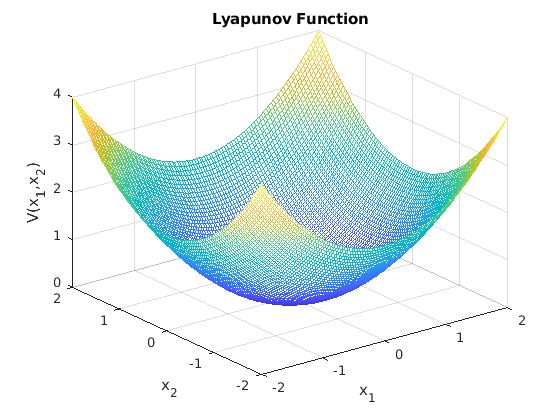
\includegraphics[width=\textwidth]{figures/lab6_1_lyapunov.png}
	\caption{Função de Lyapunov utilizada.}
    \end{subfigure}
    \begin{subfigure}{0.45\textwidth}
	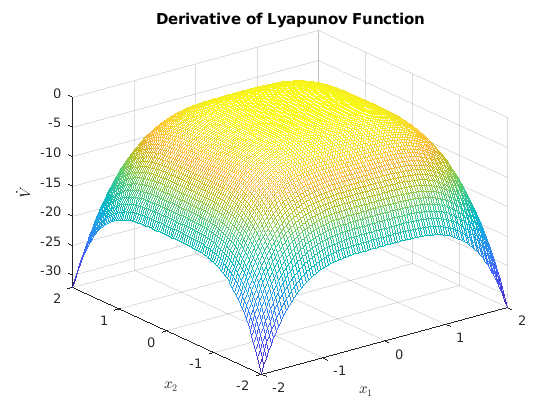
\includegraphics[width=\textwidth]{figures/lab6_1_dot_lyapunov.png}
	\caption{Derivada em relação ao tempo da função de Lyapunov.}
    \end{subfigure}
    \caption{Comportamento da função de Lyapunov utilizada em relação aos estados.}
    \label{fig:figures-lab4_1_resposta_simulink}
\end{figure}

Assim, analisamos a função matematicamente para confirmar a nossa intuição. Temos \[
\dot{V}\left( \bm{x} \right)  = \nabla V \cdot f\left( \bm{x} \right)
\], onde $f( \bm{x}) = \dot{\bm{x}}$ é a função que caracteriza o sistema. Temos que \[
\nabla V = \begin{bmatrix} x_1 & x_2 \end{bmatrix} 
\] e, assim, \[
\dot{V}\left( \bm{x} \right) = -x_1^{4} - x_2x_1 + x_1x_2 - x_2^{4} = -x_1^{4} - x_2^{4}
\], que é claramente negativa definida para o ponto de equilíbrio do sistema. Portanto, podemos concluir que o ponto de equilíbrio é assintoticamente estável.

Verificamos o resultado através do software \emph{pplane8}. Os resultados são vistos na figura \ref{fig:figures-lab6_1_pplane-png}. Vemos que o sistema converge para o ponto de equilíbrio de todas as direções.

\begin{figure}[H]
    \centering
    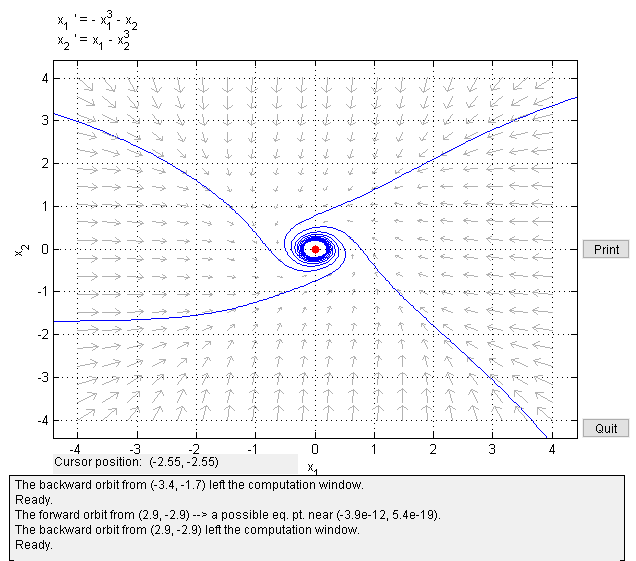
\includegraphics[width=0.6\textwidth]{figures/lab6_1_pplane.png}
    \caption{Espaço de estados do primeiro sistema.}
    \label{fig:figures-lab6_1_pplane-png}
\end{figure}

\exercise{E2}

Dado o sistema \[
\begin{cases}
    \dot{x}_1 = x_1\left( x_1^2+x_2^2-1 \right) -x_2 \\
    \dot{x}_2 = x_2\left( x_1^2+x_2^2 -1 \right) +x_1
\end{cases}
\], encontramos o único ponto de equilíbrio que é o ponto de equilíbrio trivial.

Podemos linearizar o sistema no ponto de equilíbrio, de tal fora que ele se torne \[
\bm{\dot{x}} = A\bm{x}
\], onde $A$ é a matriz jacobiana do sistema não linear avaliada no ponto de equilíbrio, ou seja, \[
A = \begin{bmatrix} \left( x_1^2+x_2^2 -1 \right) + 2x_1^2 & x_1\left( 2x_2 \right)  -1 \\ x_2\left( 2x_1 \right) +1 & \left( x_1^2+x_2^2 -1 \right) + 2x_2^2  \end{bmatrix} = \begin{bmatrix} -1 & -1 \\ 1 & -1 \end{bmatrix} 
\] o que implica em autovalores \[
det\left( \lambda I - A \right) \implies \lambda = -1 \pm j
\], portanto o equilíbrio é estável.

Ainda assim, utilizando a função de Lyapunov \[
V\left( \bm{x} \right) =\frac{1}{2} \|\bm{x}\|
\] validamos a estabilidade do sistema. Podemos determinar a função \[
\dot{V}\left( \bm{x} \right) = x_1^2\left( x_1^2+x_2^2 -1 \right) -x_1x_2 + x_2^2\left( x_1^2+x_2^2 -1 \right) + x_1x_2 = \left( x_1^2 + x_2^2 \right) \left( x_1^2+x_2^2 -1 \right)
\], que é negativa somente quando $\|\bm{x}\|<1$. Assim, concluímos que o ponto de equilíbrio é localmente estável, somente dentro do círculo unitário.

Verificamos nosso resultado em relação à característica de $\dot{V}\left( \bm{x} \right) $ de forma gráfica. O resultado pode ser observado na figura \ref{fig:figures-lab6_2_dot_lyapunov-png}. Observamos que a função de fato só se torna negativa dentro do circulo unitário.

\begin{figure}[H]
    \centering
    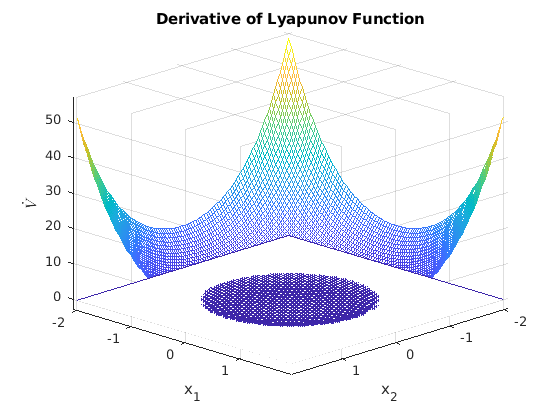
\includegraphics[width=0.6\textwidth]{figures/lab6_2_dot_lyapunov.png}
    \caption{Derivada da função de Lyapunov utilizada no segundo sistema.}
    \label{fig:figures-lab6_2_dot_lyapunov-png}
\end{figure}

Validamos nosso resultado através do software \emph{pplane}. O resultado pode ser observado na figura \ref{fig:figures-lab6_2_pplane-png}. Vemos que o sistema converge para o ponto de equilíbrio a partir do circulo unitário, enquanto a tendência dos estados, anotada pelas flechas no gráfico, mostram que o sistema diverge para estados fora do círculo unitário.

\begin{figure}[H]
    \centering
    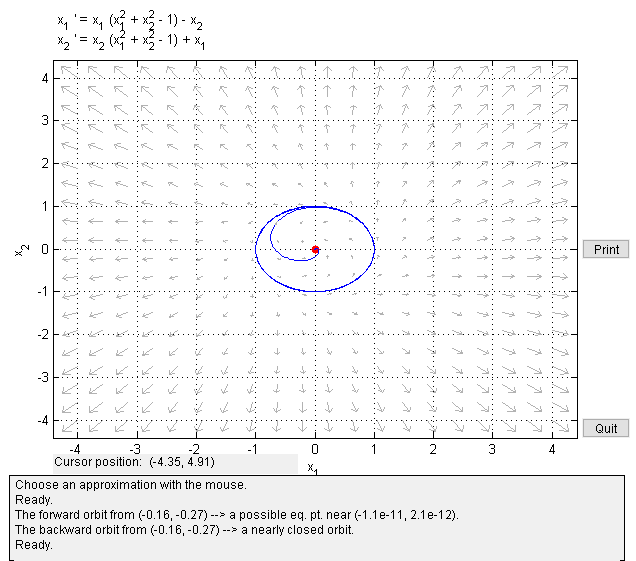
\includegraphics[width=0.6\textwidth]{figures/lab6_2_pplane.png}
    \caption{Espaço de estados do segundo sistema}
    \label{fig:figures-lab6_2_pplane-png}
\end{figure}

\exercise{E3}

Dado o sistema \[
\begin{cases}
    \dot{x}_1 = x_1x_2 \\
    \dot{x}_2 = -x_1^2 - x_2^{3}
\end{cases}
\], vemos que, claramente, o ponto de equilíbrio trivial é o único do sistema.

Agora, utilizando \[
    V\left( \bm{x} \right) = \frac{1}{2}\|\bm{x}\|
\] podemos observar que \[
\dot{V}\left( \bm{x} \right) = x_1^2x_2 - x_1^2x_2-x_2^{4} = - x_2^{4}
\], portanto negativa semi-definida, uma vez que é nula para todos os pontos $\bm{x} = \begin{bmatrix} x_1 & 0 \end{bmatrix}^{T}$. Ou seja, podemos concluir somente a estabilidade do sistema. Podemos verificar esse resultado de forma gráfica através da figura \ref{}.

\begin{figure}[H]
    \centering
    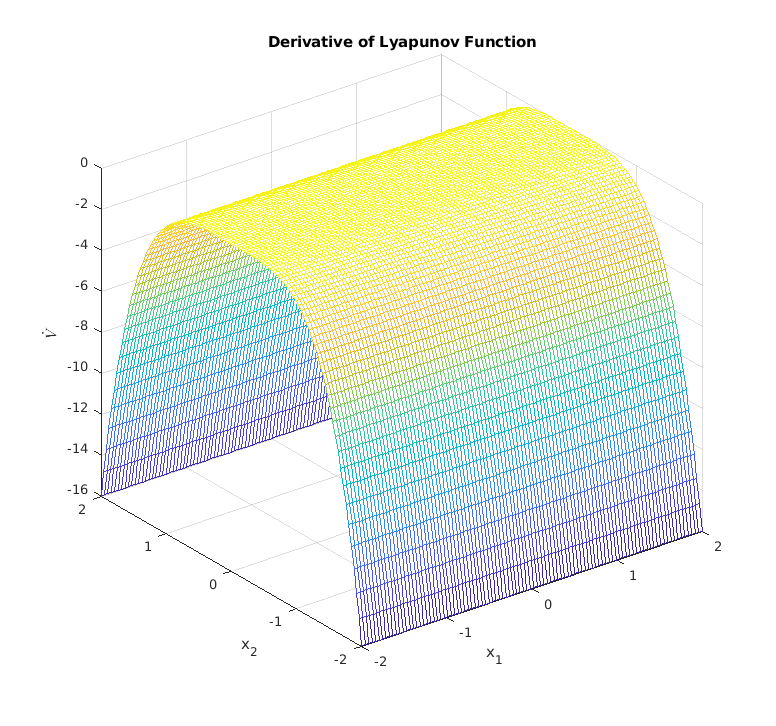
\includegraphics[width=0.6\textwidth]{figures/lab6_3_dot_lyapunov.png}
    \caption{Derivada da função de Lyapunov utilizada no terceiro sistema.}
    \label{fig:figures-lab6_3_dot_lyapunov-png}
\end{figure}

Entretanto, analisando o sistema para a condição encontrada, temos que
\begin{align*}
& \lim_{x_2 \to 0} \dot{x}_2 = 0 \\
& \implies \lim_{x_2 \to 0} -x_1^2 - x_2^{3} = 0 \\
& \implies \lim_{x_2 \to 0} x_1 = 0
\end{align*}
, ou seja, o sistema converge para o ponto de equilíbrio e, portanto, é assintoticamente estável.

Verificamos esse resultado utilizando o software \emph{simulink} para simular a resposta do sistema com 4 condições iniciais diferentes, conforme na figura \ref{fig:figures-lab6_3_pplane-png}. Vemos que o sistema converge para o ponto de equilíbrio em todos os casos, conforme esperado.

\begin{figure}[H]
    \centering
    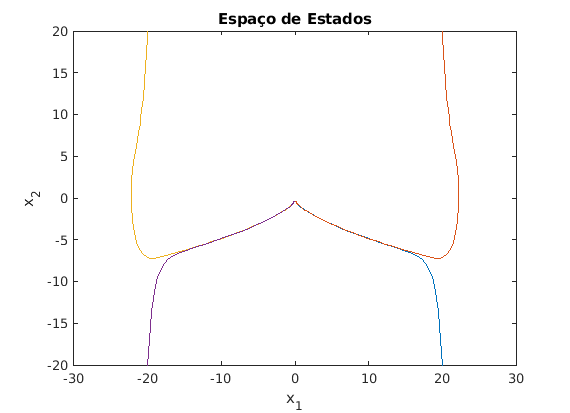
\includegraphics[width=0.6\textwidth]{figures/lab6_3_state_space.png}
    \caption{Espaço de estados do terceiro sistema com algumas trajetórias simuladas.}
    \label{fig:figures-lab6_3_pplane-png}
\end{figure}

\end{document}
